\documentclass[UTF8,a4paper,12pt, onecolumn]{ctexart}
\usepackage[left=2.50cm, right=2.50cm, top=2.50cm, bottom=2.50cm]{geometry}

% -- text font --
% compile using Xelatex

%\setmainfont{Microsoft YaHei}  % 微软雅黑
%\setmainfont{YouYuan}  % 幼圆    
%\setmainfont{NSimSun}  % 新宋体
%\setmainfont{KaiTi}    % 楷体
\setmainfont{Songti SC}   % 宋体
%\setmainfont{SimHei}   % 黑体

\usepackage{times}
%\usepackage{mathpazo}
%\usepackage{fourier}
%\usepackage{charter}
%\usepackage{helvet}

\usepackage{amsmath, amsfonts, amssymb} % math equations, symbols
%\usepackage[english]{babel}
\usepackage{color}      % color content
\usepackage{graphicx}   % import figures
\usepackage{url}        % hyperlinks
\usepackage{bm}         % bold type for equations
\usepackage{multirow}
\usepackage{booktabs}
\usepackage{epstopdf}
\usepackage{epsfig}
\usepackage{algorithm}
\usepackage{algorithmic}
\renewcommand{\algorithmicrequire}{ \textbf{Input:}}     % use Input in the format of Algorithm  
\renewcommand{\algorithmicensure}{ \textbf{Initialize:}} % use Initialize in the format of Algorithm  
\renewcommand{\algorithmicreturn}{ \textbf{Output:}}     % use Output in the format of Algorithm  

\usepackage{fancyhdr}   % 设置页眉、页脚
%\pagestyle{fancy}
\lhead{}
\chead{}
%\rhead{\includegraphics[width=1.2cm]{}}
\lfoot{}
\cfoot{}
\rfoot{}

\usepackage{gbt7714}
%\renewcommand{\refname}{参考文献}   % 将References改为参考文献

%\usepackage{draftwatermark}         % 所有页加水印
%\usepackage[firstpage]{draftwatermark} % 只有第一页加水印
%\SetWatermarkText{Water-Mark}           % 设置水印内容
%\SetWatermarkText{\includegraphics{}}         % 设置水印logo
%\SetWatermarkLightness{0.9}             % 设置水印透明度 0-1
%\SetWatermarkScale{1}                   % 设置水印大小 0-1    

\usepackage{hyperref}   % bookmarks
\hypersetup{colorlinks, bookmarks, unicode} % unicode
\usepackage{pdfpages}

\title{血液疾病辅助诊断方法研究}
\author{}
\date{\today}


\begin{document}
    \maketitle
    \thispagestyle{fancy}
    
\tableofcontents

\section{背景介绍}

血液病是原发于造血系统的疾病,或影响造血系统伴发血液异常改变,以贫血、出血、发热为特征的疾病。造血系统包括血液、骨髓单核一巨噬细胞系统和淋巴组织,凡涉及造血系统病理、生理,并以其为主要表现的疾病,都属于血液病范畴。

目前,引起血液病的因素很多,诸如:化学因素、物理因素、生物因素、遗传、免疫、污染等,都可以成为血液病发病的诱因或直接原因,由于这些原因很多是近几十年现代工业的产物,从而使血液病的发病率有逐年增高的趋势,可以说,血液病是一种现代病。

血液病临床分为三大类型:红细胞疾病、白细胞疾病、出血和血栓性疾病。临床上常见的疾病有白血病、再生障碍性贫血、骨髓增生异常综合症、血小板减少症、多发性骨髓瘤、淋巴瘤、骨骼纤维化、血友病、地中海贫血等。

血液病常用的检查包括:血常规、血细胞形态学检查、白细胞分类、骨髓细胞分析、血细胞化学染色、染色体核型检查、免疫学检查、骨髓病理活检、相关酶学检查等等。其中,血常规是最一般,最基本的血液检验,也是常规体检中必包含的检验项目。

血常规是指通过观察血细胞的数量变化及形态分布从而判断血液状况及疾病的检查,随着检验现代化、自动化的发展,现在的血常规检验是由机器检测完成的。血液由液体和有形细胞两大部分组成,血常规检验的是血液的细胞部分。血常规检查包括有红细胞计数(RBC)、血红蛋白(Hb)、白细胞(WBC)、白细胞分类计数及血小板(PLT)等,通常可分为三大系统,即红细胞系统、白细胞系统和血小板系统。通过观察数量变化及形态分布,判断疾病。血常规中的许多项具体指标都是一些常用的敏感指标,对机体内许多病理改变都有敏感反映,其中又以白细胞计数、红细胞计数、血红蛋白和血小板最具有诊断参考价值,许多患者在病因不明时可以做血常规检查对其进行辅助诊断,是医生诊断病情的常用辅助检查手段之一。此外,血常规检查还是观察治疗效果、用药或停药、继续治疗或停止治疗、疾病复发或痊愈的常用指标。

目前,大数据平台收集整理了约150万例的血常规检验数据,经过对血常规数据的统计分析,最终整理出了22个血常规指标项,基于这部分数据集,运用机器学习等技术,构建针对主要血液疾病的初步诊断模型,并在临床实践中对诊断模型进行验证,待诊断模型改进优化后向县级等基层医疗机构进行推广,实现血液疾病的初步筛选,减轻专业型医院的就诊压力。

\section{解决方案}

通过对原始数据及诊断结果的分析,汇总出了22个血常规指标项(如表\ref{tb:22metrics})和九类发病率比较高的血液疾病,九类高发病率血液疾病及对应的病例数如表\ref{tb:9boold}所示。

\begin{table}
\centering
\begin{tabular}{|l|l|}
\toprule
\multicolumn{2}{|c|}{血常规指标项} \\
\midrule
白细胞		&	血小板计数	\\
淋巴细胞计数	&	嗜酸性粒细胞计数	\\
红细胞压积	&	单核细胞比率	\\
平均血小板体积	&	红细胞分布宽度	\\
平均血红蛋白浓度	&	淋巴细胞比率	\\
血红蛋白		&	嗜碱性粒细胞比率	\\
中性粒细胞计数	&	嗜酸性粒细胞比率	\\
平均血红蛋白含量	&	中性粒细胞比率	\\
单核细胞计数	&	血小板分布宽度	\\
嗜碱性粒细胞计数	&	红细胞计数	\\
血小板压积	&	红细胞平均体积	\\
\bottomrule
\end{tabular}
\caption{22个血常规指标项}
\label{tb:22metrics}
\end{table}

\begin{table}
\centering
\begin{tabular}{|l|l|l|}
\toprule
\multicolumn{3}{|c|}{血常规指标项(正负样本字段)} \\
\midrule
原血液病数据字段	&	指标项意义	&	统一字段名 \\
\midrule
var\_565	 & 	平均血红蛋白含量	 & 	MCH	\\
var\_493	 & 	平均血红蛋白浓度	 & 	MCHC	\\
var\_835	 & 	红细胞平均体积	 & 	MCV	\\
var\_447	 & 	平均血小板体积	 & 	MPV	\\
var\_640	 & 	嗜碱性粒细胞计数	 & 	BAS	\\
var\_828	 & 	嗜碱性粒细胞比率	 & 	BAS\_P	\\
var\_764	 & 	嗜酸性粒细胞计数	 & 	EOS	\\
var\_514	 & 	血红蛋白	 & 	HB	\\
var\_832	 & 	血小板分布宽度	 & 	PDW	\\
var\_739	 & 	血小板计数	 & 	PLT	\\
var\_829	 & 	嗜酸性粒细胞比率	 & 	EOS\_P	\\
var\_119	 & 	白细胞计数	 & 	WBC	\\
var\_831	 & 	中性粒细胞比率	 & 	NEUT\_P	\\
var\_559	 & 	中性粒细胞计数	 & 	NEUT	\\
var\_660	 & 	血小板压积	 & 	PCT	\\
var\_826	 & 	红细胞分布宽度	 & 	RDW	\\
var\_183	 & 	淋巴细胞计数	 & 	LY	\\
var\_827	 & 	淋巴细胞比率	 & 	LY\_P	\\
var\_599	 & 	单核细胞计数	 & 	MONO	\\
var\_834	 & 	红细胞计数	 & 	RBC	\\
var\_825	 & 	单核细胞比率	 & 	MONO\_P	\\
var\_40	 & 	红细胞压积	 & 	HCT	\\
性别	 & 	性别	 & 	Sex	\\
年龄	 & 	年龄	 & 	Age \\
\bottomrule
\end{tabular}
\end{table}


\begin{table}
\centering
\begin{tabular}{|l|r|}
\toprule
血液疾病 & 病例数  \\ 
\midrule
淋巴瘤 & 5976   \\ 
\hline
多发性骨髓瘤[卡勒病] (M97320/3) & 2684   \\ 
\hline
急性髓样白血病 & 2084 \\ 
\hline
血小板减少性紫癜 & 1333 \\
\hline
过敏性紫癜[亨诺克(-舍恩莱因)紫癜] & 1169 \\
\hline
急性淋巴细胞白血病 & 1167 \\
\hline
再生障碍性贫血 NOS & 629 \\
\hline
噬血细胞综合症 & 413 \\
\hline
骨髓增生异常综合征 & 309 \\
\bottomrule
\end{tabular}
\caption{九类高发病率血液疾病}
\label{tb:9boold}
\end{table}

\subsection{预期假设}

使用机器学习的方法实现血液疾病的辅助诊断,基于以下假设前提:

\begin{enumerate}
  \item 假设22个血常规指标与9类高发病率血液疾病有相关关系,即通过22个指标数据就可以推断是血液类疾病。
  \item 假设9类高发病率血液疾病在血检指标上有明显的区别,即通过22个指标数据能明确推断是哪类血液疾病。
\end{enumerate}

假设否定:

\begin{enumerate}
  \item 基于22个指标数据,通过机器学习方法无法准确判断正负样本,即无法准确区分患病与正常病例,则表明通过22个指标数据,并不能在临床上准确诊断是否患血液病,这种情况下,需要考虑增加指标。
  \item 基于22个指标数据,通过机器学习方法可以准确区分患病与正常病例,但是对于某两类疾病的区分准确率较低,则表明22个指标数据在临床上不能诊断这两类疾病。
\end{enumerate}



\subsection{数据预处理}

数据平台中的体检数据来自多个数据源,各数据源之间数据标准不一致,比如血常规指标项对应的字段名称不一致、数据单位不一致等,另外还存在部分指标项缺失的情况,所以,首先需要对数据进行预处理。

\subsubsection{字段名称不一致}

需要在临床专业医生的指导下,建立字段名称对应关系,然后将数据统一映射到标准字段名称下。

\subsubsection{处理缺失指标项}

数据缺失有三种情况:完全随机缺失(Missing completely at random (MCAR))、随机缺失(Missing at random (MAR))、不可忽略的缺失(Not missing at random (NMAR))。

主要有6种处理数据缺失的方法:

\begin{enumerate}
	\item 不作处理。对于某些算法可以处理数据缺失的情况, 例如:XGBoost算法可以基于训练数据估算缺失值;LightGBM算法有忽略缺失值的参数选项。但是,某些算法不能接受数据缺失,例如:Scikit的LinearRegression算法。
	\item 使用均值或中值填补。
	\begin{itemize}
		\item 优点
		\begin{itemize} 
			\item 简单快速
			\item 适用于小的数值数据集
		\end{itemize}
		\item 缺点
		\begin{itemize}
			\item 只适用列级别,没有考虑特征之间的相关性
			\item 不能用于分类特征
			\item 不是很准确
			\item 没有说明估算的不确定性
		\end{itemize}
	\end{itemize}
	\item 使用最高频率值或0或常量填补
	\begin{itemize}
		\item 优点
		\begin{itemize}
		\item 非常适用于分类特征
		\end{itemize}
		\item 缺点
		\begin{itemize}
  			\item 没有考虑特征之间的相关性
  			\item 在数据中引入偏差
		\end{itemize}
	\end{itemize}
	\item 使用K近邻方法填补。
	\begin{itemize}
		\item 优点
		\begin{itemize}
		  \item 比均值、中值或最高频率估算方法更加准确
		\end{itemize}
		\item 缺点
		\begin{itemize}
		  \item 计算代价大,因为KNN需要在内存中保存整个训练数据。
		  \item K-NN对数据中的异常值(Outliers)非常敏感。
		\end{itemize}
	\end{itemize}
	\item 使用链式方程多元插值(Multivariate Imputation by Chained Equation (MICE))\cite{buuren2010mice}((参见附录\ref{pdf:mice}))
	\begin{itemize}
		\item 优点 
		\begin{itemize}
		  \item 灵活,可以处理不同数据类型(ie., continuous or binary)的不同变量
		\end{itemize}
		\item 缺点 
	\end{itemize}
	\item 使用深度学习的方法估值(DataWig \footnote{DataWig - Imputation for Tables, https://github.com/awslabs/datawig})
	\begin{itemize}
		\item 优点
		\begin{itemize}
		  \item 适用于分类和非数值型数据
		  \item 与其它方法相比较更加准确
		  \item 提供了处理分类数据的方法, 如: Feature Encoder
		  \item 支持GPUs和CPUs
		\end{itemize}
		\item 缺点
		\begin{itemize}
		  \item 仅支持单列估算
		  \item 处理大数据集, 计算时间长.
		  \item 需要手动关联与被估算列信息相关的其它列.
		\end{itemize}

	\end{itemize}
\end{enumerate}

综上所述,没有完美的方法来补偿数据集中的缺失值。 每种策略对于某些数据集和缺失的数据类型都可以表现更好,但在其他类型的数据集上可能会表现得更差。 有一些设置规则可以决定使用哪种策略来处理特定类型的缺失值,但除此之外,可以尝试并检查哪种模型最适合当前的数据集。

针对血常规检验的指标特点,可以采用正常值填补缺失值。但是,在对缺失数据进行估算之前, 必须先处理异常值。

\subsection{采样(随机)}

数据完成预处理后,需要针对机器学习的训练任务,对数据通过采样的方法获取训练数据。目前,采样中遇到的最大问题是正负样本数据的不平衡,而造成这个问题的主要原因是部分血液疾病在人群中的患病率太低。

\subsubsection{不平衡样本问题(Imbalanced Data)}

不平衡数据通常是指分类问题的问题,其中分类没有被平等地表示。例如,可能有一个包含100个实例(样本)的二分类问题,总共80个实例标记为负样本,其余20个实例标记为正样本。这是一个不平衡的数据集,正负样本的比例为80:20或4:1。对于二分类问题以及多分类问题,都可能会遇到分类不平衡问题。

处理正负样本数据不平衡的问题,主要有以下解决方法 \footnote{\href{https://machinelearningmastery.com/tactics-to-combat-imbalanced-classes-in-your-machine-learning-dataset/}{8 Tactics to Combat Imbalanced Classes in Your Machine Learning Dataset}} 。

\begin{enumerate}
  \item 采集更多的数据。
  \item 改变性能评价指标\footnote{\href{https://machinelearningmastery.com/classification-accuracy-is-not-enough-more-performance-measures-you-can-use/}{Classification Accuracy is Not Enough: More Performance Measures You Can Use}}。
	\begin{enumerate}
	  \item 识别率(Accuracy)。$ Acc = \frac{N_{pre}}{N_{total}} $, $N_{pre}$表示预测对的样本数, $N_{total}$表示测试集总的样本数。
	  \item 混淆矩阵(Confusion Matrix)(参见附录\ref{pdf:Confusion_matrix})。又称为可能性表格或是错误矩阵,是一种特定的矩阵用来呈现算法性能的可视化效果,通常是监督学习(非监督学习,通常用匹配矩阵:matching matrix)。其每一列代表预测值,每一行代表的是实际的类别。
	  \item 命中率(Precision)。命中率=正确预测到的正例数/预测正例总数。$ Precision = \frac{TP}{TP+FP}$
	  \item 覆盖率(Recall)。覆盖率=正确预测到的正例数/实际正例总数。$ Recall = \frac{TP}{P} $
	  \item F1 Score(参见附录\ref{pdf:F1})。$F1=\frac{2TP}{2TP+FN+FP}=\frac{2 \cdot Precision \cdot Recall}{Precision+Recall}$
	  \item 分类回归树(Classification and Regression Tree,CART)(参见附录\ref{pdf:cart}).
	  \item Kappa(参见附录\ref{pdf:Kappa}).
	  \item ROC曲线(接收者操作特征)和AUC(Area under Curve)值(参见附录\ref{pdf:roc})。ROC曲线有个很好的特性:当测试集中的正负样本的分布变换的时候,ROC曲线能够保持不变。在实际的数据集中经常会出现样本类不平衡,即正负样本比例差距较大,而且测试数据中的正负样本也可能随着时间变化。
	  
	\end{enumerate}

  \item 对数据进重采样。
	\begin{itemize}
	  \item 过采样
	  \begin{itemize}
		  \item 随机过采样
		  \item SMOTE(Synthetic Minority Over-sampling Technique)
		  \item ADASYN
		\end{itemize}
	  \item 欠采样
	\end{itemize}

  \item 尝试生成合成样本。即SMOTE。
  \item 尝试不同的算法。
  \item 尝试使用惩罚模型(Penalized Models)。
\end{enumerate}

统计学检验方法:

\begin{itemize}
  \item 卡方检验(Chi square test),实际观测值与理论(模型)推断值偏离程度
  \item KS test, 比较频率分布与理论(模型)分布偏离程度
  \item PSI指数(相对熵),脱胎于Kullback-Leibler散度(Kullback-Leibler divergence)或信息散度(information divergence). 相对熵表示使用理论分布拟合真实分布时产生的信息损耗,一般认为psi小于0.1时候模型稳定性很高,0.1-0.25一般,大于0.25模型稳定性差,建议重做。psi = sum((实际占比-预期占比)/ln(实际占比/预期占比))
\end{itemize}

\subsection{机器学习模型}

\subsubsection{逻辑回归(Logistic Regression)}

\subsubsection{随机森林(Random Forest)}

\subsubsection{Light GBM}

\subsubsection{XGBoost}

\subsubsection{神经网络(NN)}

\subsection{模型训练}

逻辑回归是重要的benchmark,后面的算法表现还不如它肯定是大有问题。同时,可以用这个模型来做一次快速诊断。诊断步骤如下:
\begin{itemize}
  \item 研究cost function的表现:如果随着训练集上的代价函数下降而交叉验证集合上却上升,就有过拟合的风险;若果训练集上下降的不好,有欠拟合的风险。
  \item 研究学习曲线:即代价函数/误差与训练样本量的函数。很容易通过图像看出欠拟合与过拟合的问题。往往一开始能弄出过拟合就行了,后面再调。
\end{itemize}

模型检验法则:
\begin{itemize}
  \item 更多的样本、更少的特征、增大惩罚项都能缓解过拟合的问题。
  \item 更多的特征、多项式特征、减少惩罚项可以处理欠拟合的问题。
  \item 模型选择要权衡偏差与方差,不可得兼。
\end{itemize}

\subsubsection{训练模型与调参}

我们把数据分成6:2:2(如果样本很大,可以减少后两者相对比例),对应训练集、交叉检验集、测试集。在训练集上训练数据,在交叉检验集上调参,最终用测试集汇报结果。

调参方法:
\begin{itemize}
  \item GridSearch
  \item RandomSearch
\end{itemize}


\bibliography{blood-references.bib}

\appendix

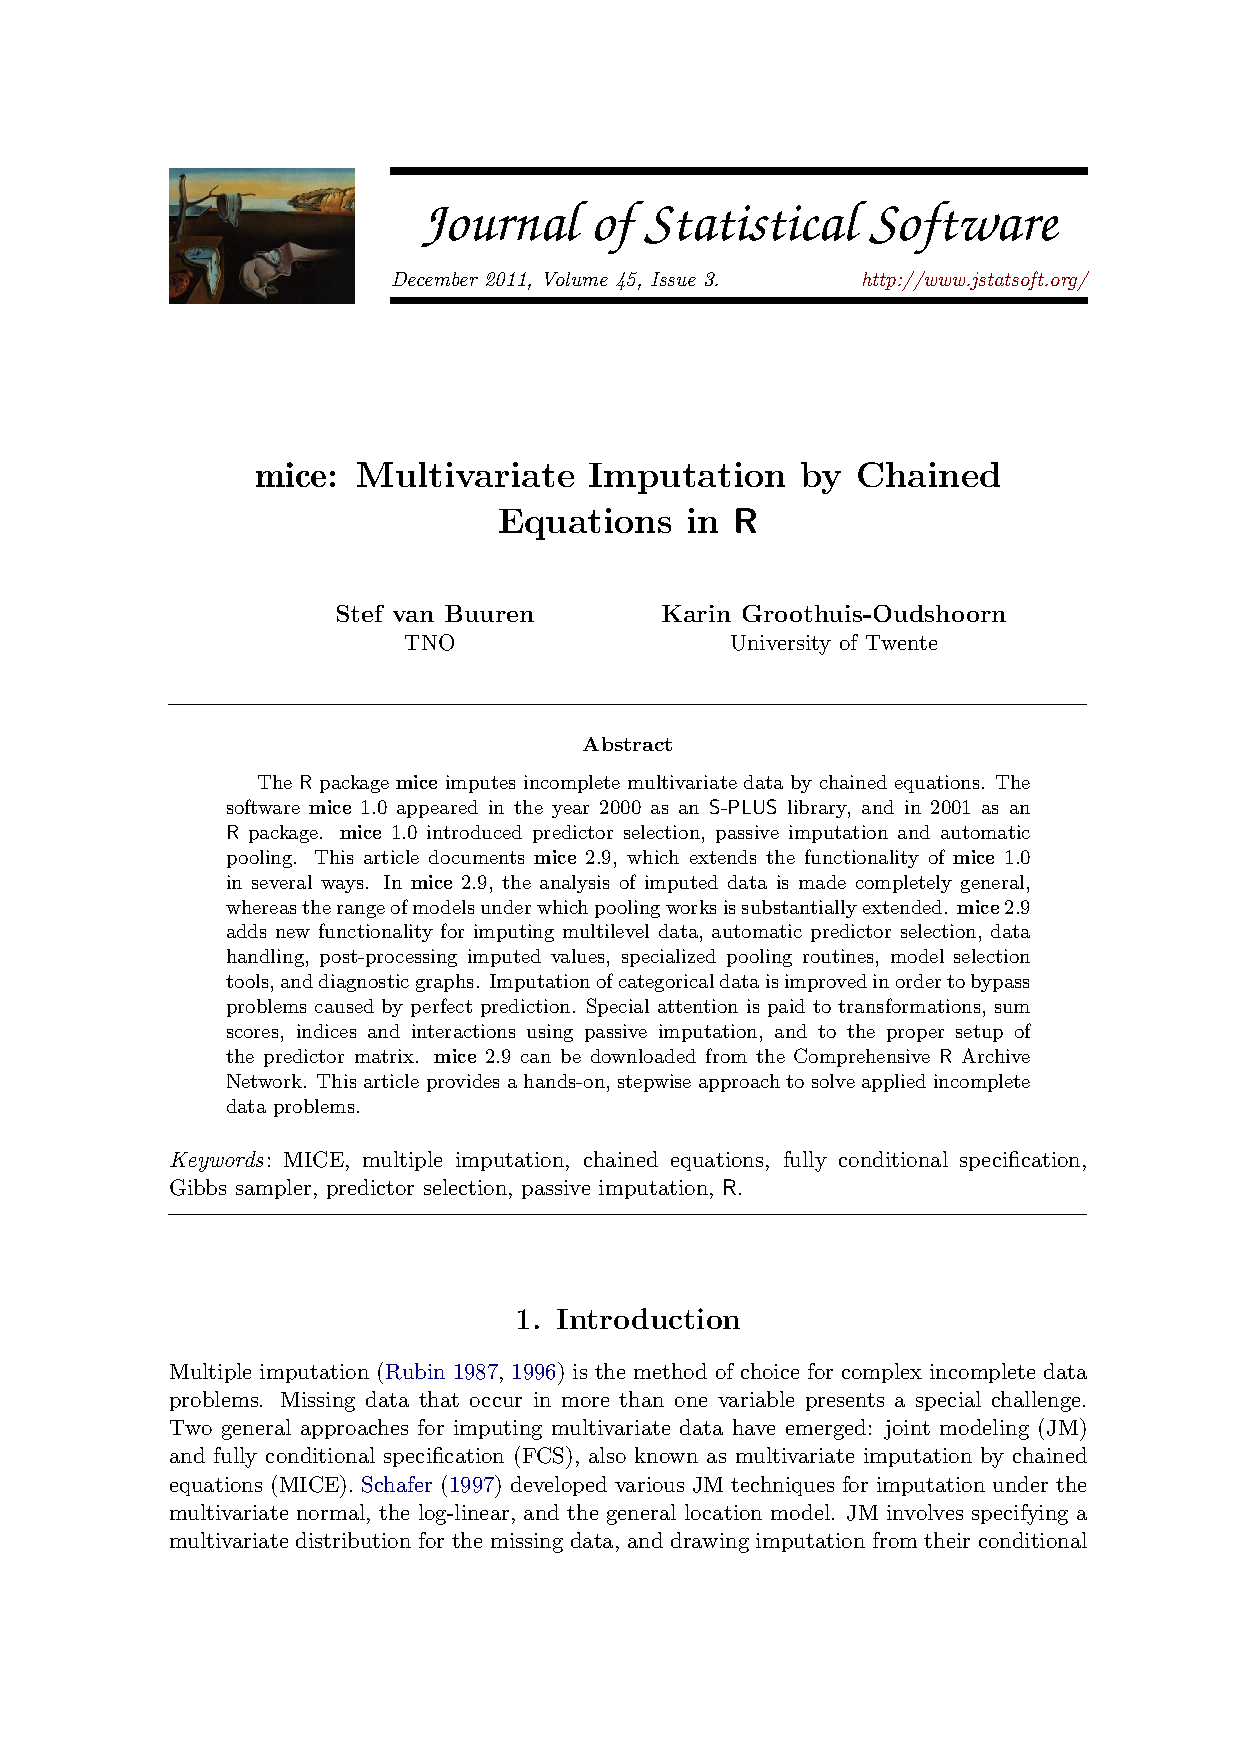
\includepdf[pages=-,addtotoc={1,section,2,MICE: Multivariate Imputation by Chained Equations in R,pdf:mice}]{v45i03}
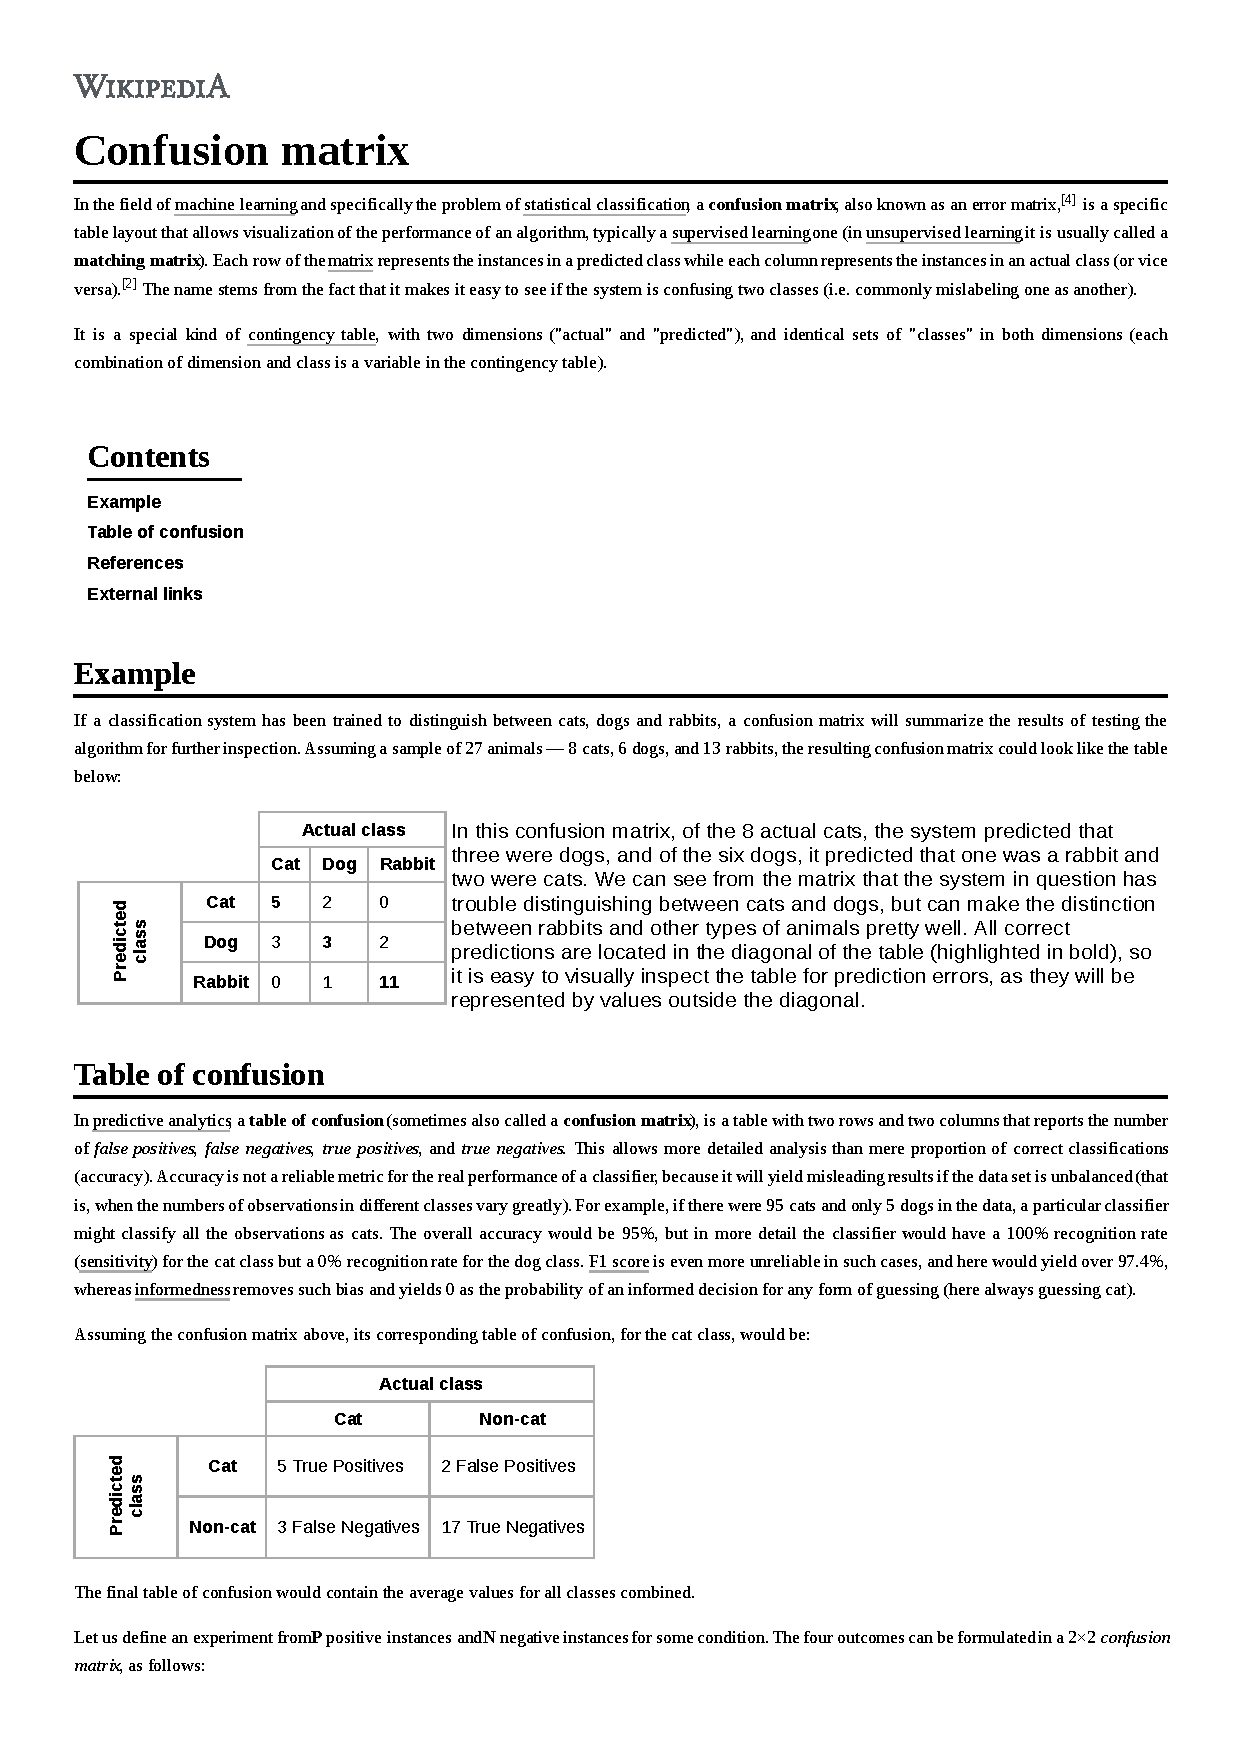
\includepdf[pages=-,fitpaper=true,addtotoc={1,section,2,Confusion Matrix,pdf:Confusion_matrix}]{Confusion_matrix}
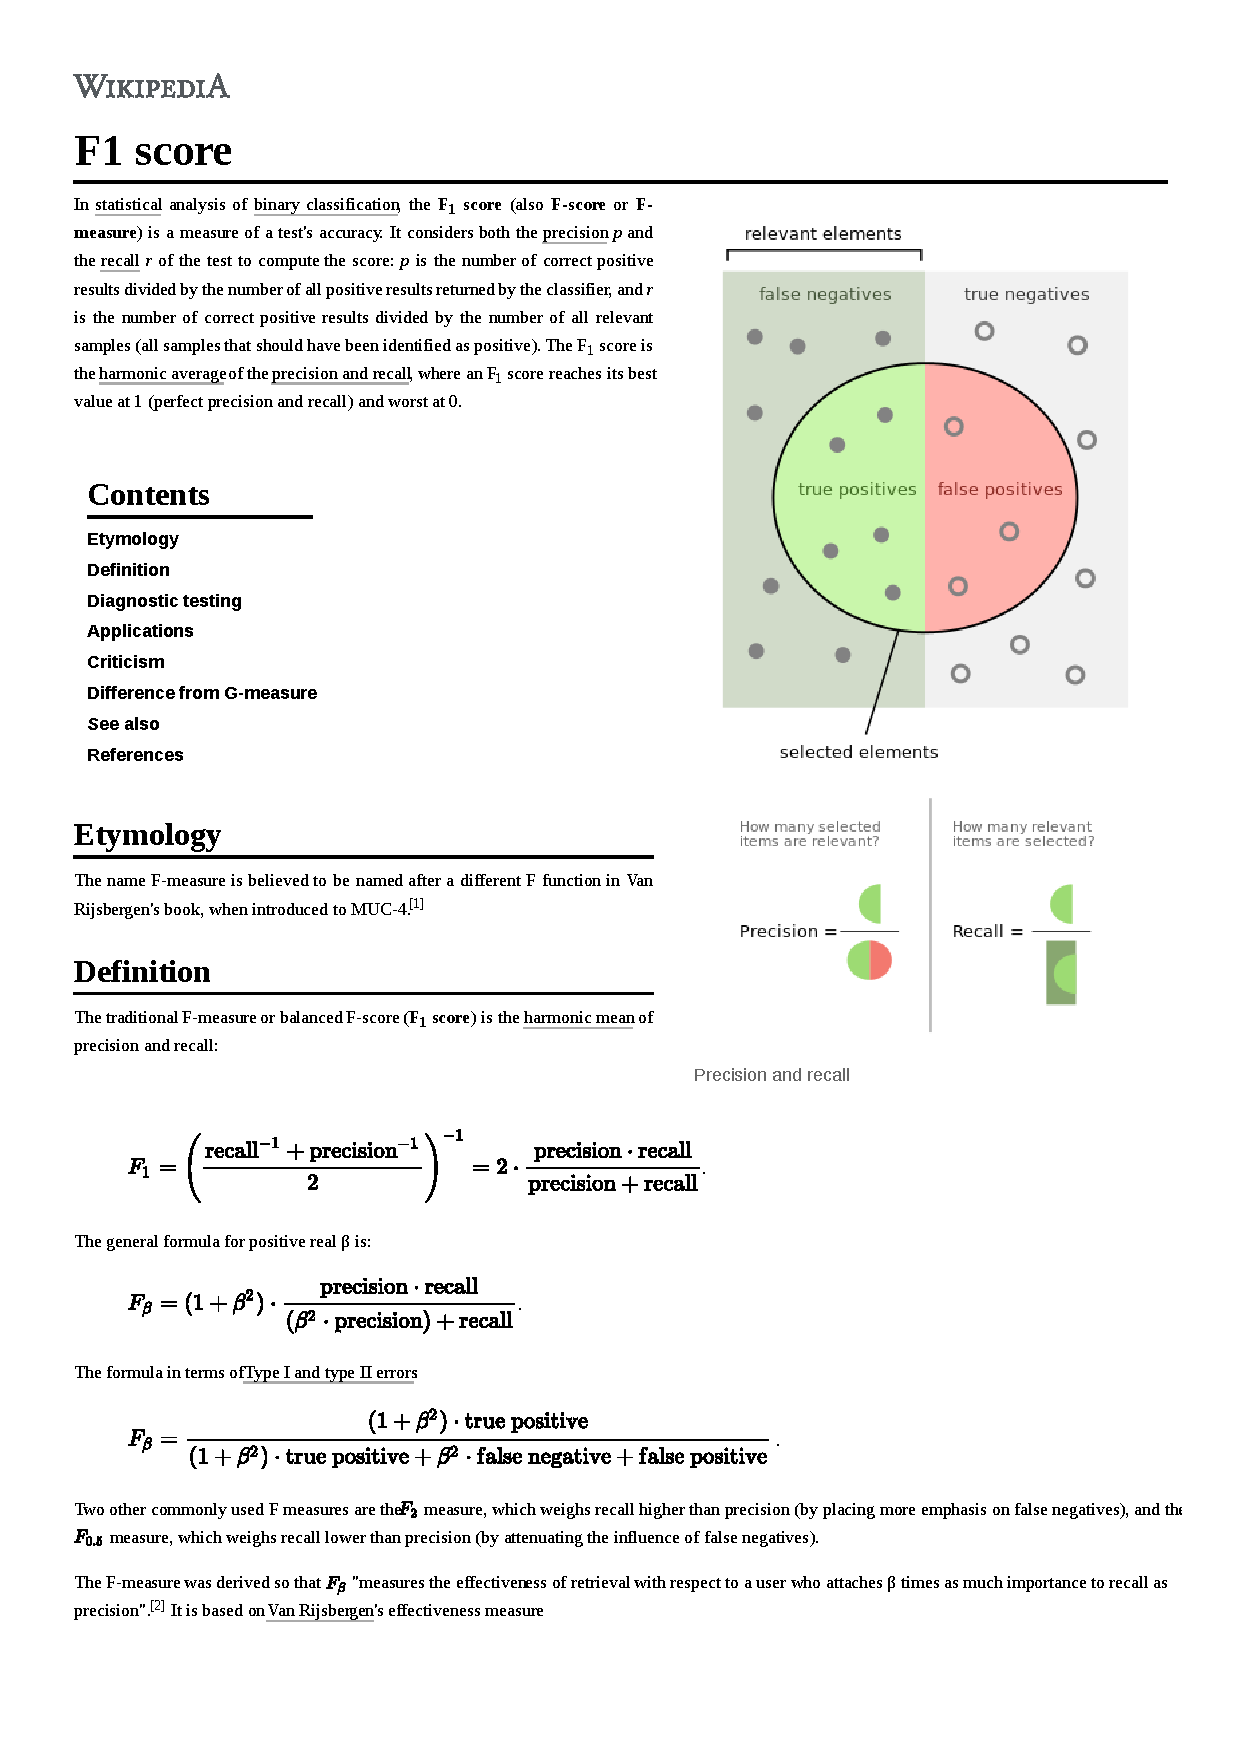
\includepdf[pages=-,fitpaper=true,addtotoc={1,section,2,F1 Score,pdf:F1}]{F1_score}
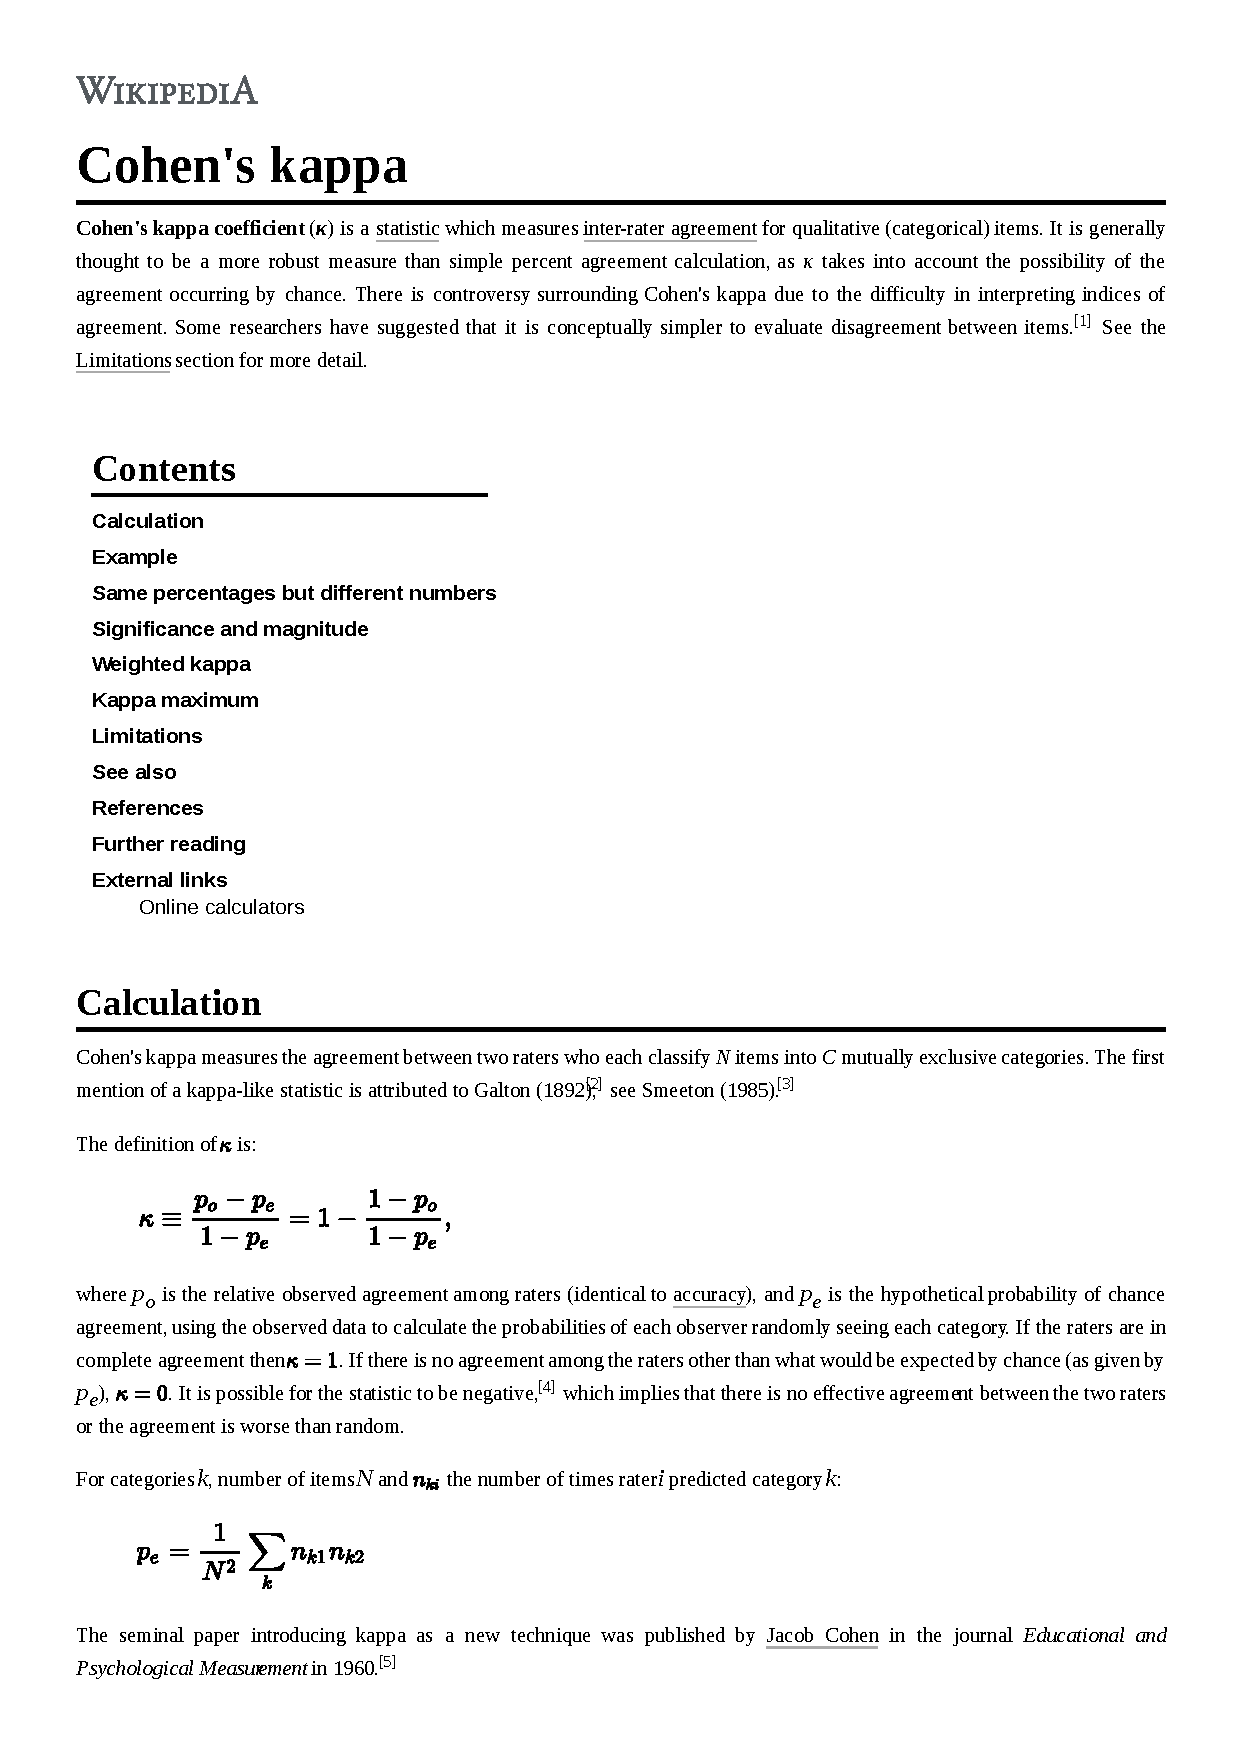
\includepdf[pages=-,fitpaper=true,addtotoc={1,section,2,Cohen's Kappa,pdf:Kappa}]{Cohen's_kappa}
\includepdf[pages=-,fitpaper=true,addtotoc={1,section,2,Receiver Operating Characteristic, pdf:roc}]{Receiver_operating_characteristic}
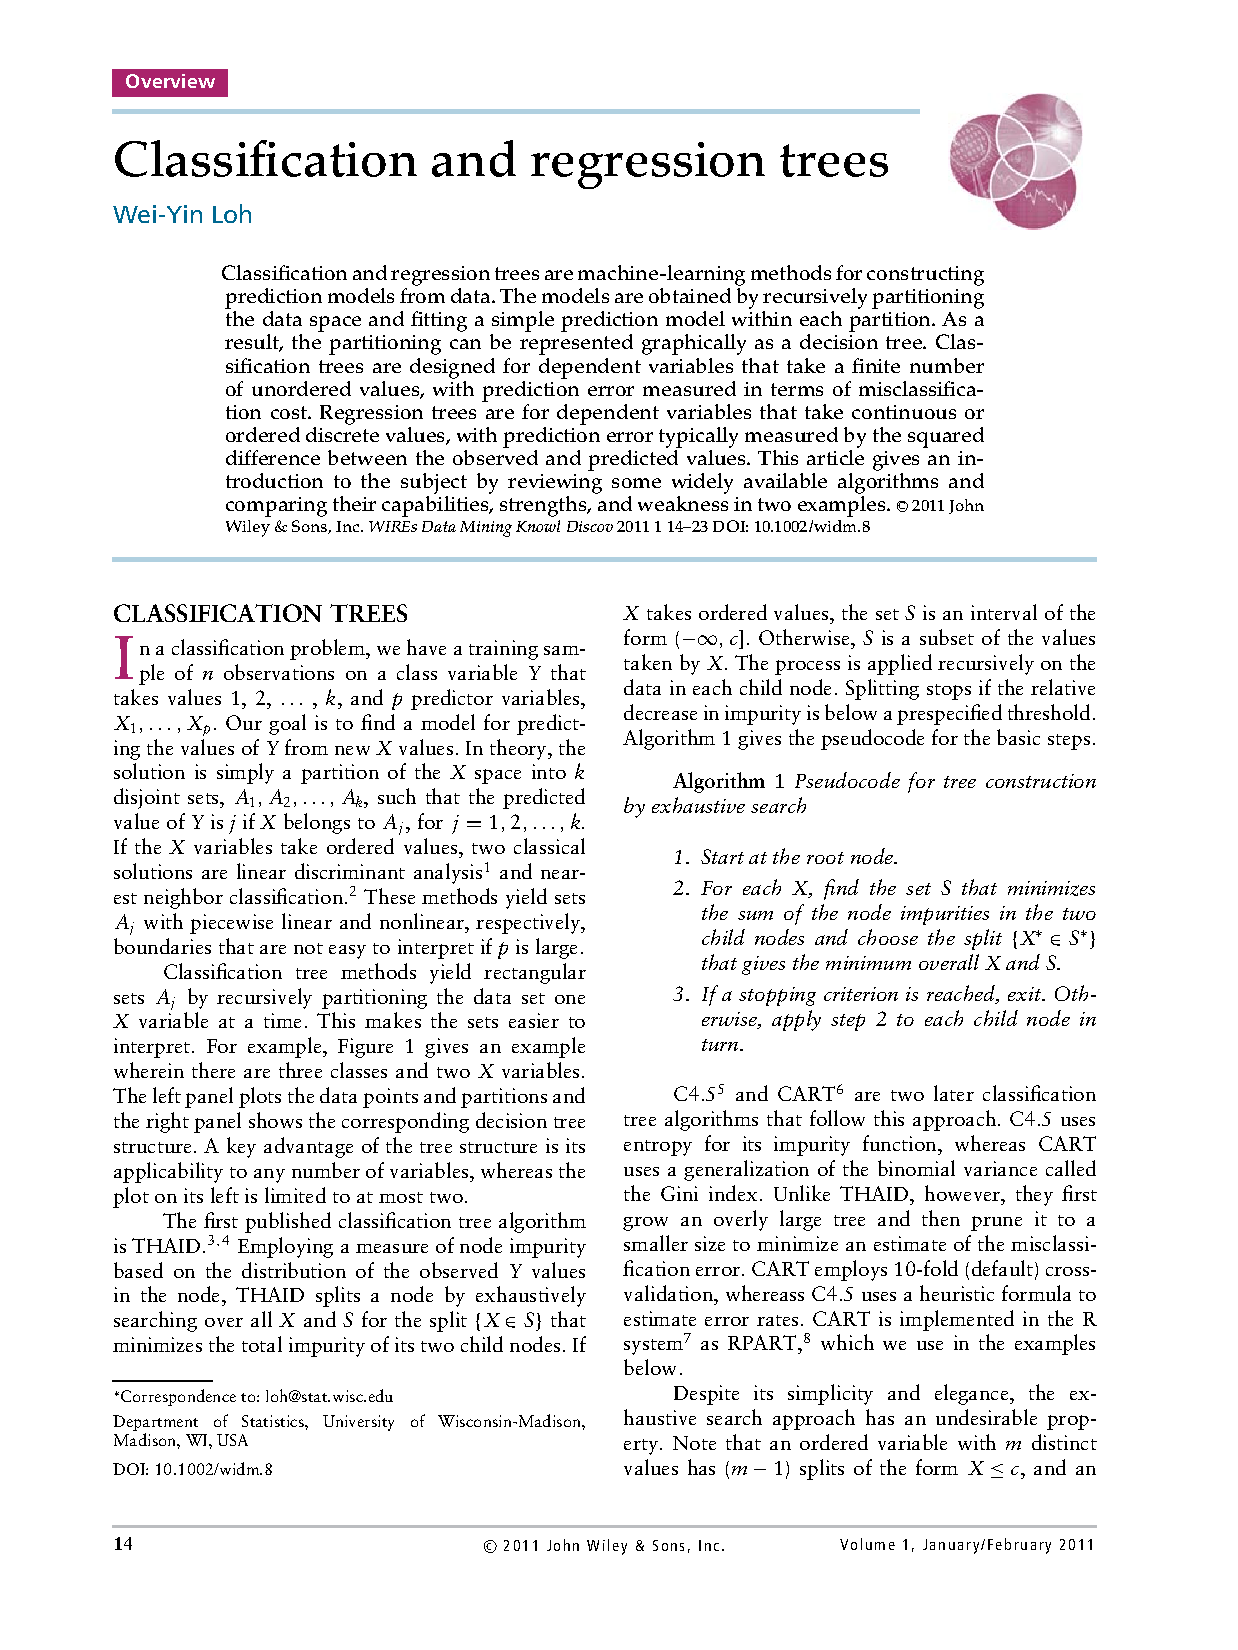
\includepdf[pages=-,addtotoc={1,section,2,Classification And Regression Trees,pdf:cart}]{wires11}
\end{document}